
\subsection{Téma választás}
Beadandóm tematikája a diplomamunkámhoz kapcsolódik melynek a tematikájául egy olyan témát fedeztem fel amely a jelenlegi munkahelyemen jelentősen megsegítené az ott dolgozók levelezési szokásait. Mivel a témát a munkahelyemről kaptam ezért, az ott dolgozók számára ez egy releváns téma volna.
A választott témában főleg arra szeretnék kitérni, hogy hogyan tudnánk megtalálni azokat a módszereket amelyek segíthetnek abban, hogy egy idősoros adaton, hogyan tudnánk kikerülni azokat az eseteket amikor a rendszer automatikusan kiküld rossz riasztásokat.
\\
Jelenleg olyan rendszer nem áll rendelkezésre a vállalatnál amely egy adatbázisrendszernél lévő idősoros adatokhoz úgy tudna határértéket igazítani, hogy az kevesebb anomáliát adjon. Továbbá, ez a határérték igazítás a jövőbeni előrejelzésnél válna a vállalat hasznára, mivel ha előre megtudnánk mondani, hogy mikor lesz nagy ingadozás a rendszerben, akkor felkészülhetnénk esetleges problémák, anomáliák sorozatára.
\\
Személy szerint én ezt a témát relevánsnak tartom mivel, benyújtást nyerhettem a vállalat riasztásának, és a belső rendszerének a működésébe.
Szeretném kifejteni azt, hogy ilyen idősoros adatokon, hogyan és miként lehetne előrejelezni értékeket, hogy azok minél közelebb álljanak a valósághoz. Továbbá, ezen előrejelzéseket, hogyan lehetne beépíteni a tesztelő és az éles rendszerbe, amely végzi ezen riasztásokat, és kiértékeléseket. Végül pedig, ezen módszer értékelése és konklúziók következtetése lesz a cél.

\subsection{Téma fontossága}
Alapvetően az a rendszer amivel a vállalat működik az adatokat, úgy tárolja, hogy abban megtalálhatóak különféle "mintázatok".

A jelenlegi rendszerben napi, heti illetve egyéb bontások alapján vannak elszeparálva az adatok. Alapvetően emögött a rendszer mögött áll egy riasztási rendszer amely, hogyha túl nagy értékeket észlel ki küldd riasztásokat levelezési szerveren keresztül. Természetesen ez a riasztás akkor is ki lesz küldve amint a beérkezett adatok, túl alacsonynak bizonyulnak. Ez a rendszer egyik legnagyobb hiányossága, hogy magát a \textit{treshold} értékét túl nagy különbségekre tudjuk beállítani.
Ez azt jelenti, hogy határértéknek a szélességét vagy túl nagyra állítjuk vagy túl alacsonyra.
Amennyiben túl nagyra állítjuk ezt az értéket, akkor amikor jelezne a rendszer a \textit{support}-nak akkora már túl nagy problémába ütköztünk. 
\\
\\
\\
Amennyiben pedig túl alacsonyra rakjuk ezt a határértéket, akkor pedig folyamatosan kiküldi az értesítéseket, ezzel azt érve el, hogy az aki figyeli ezen értékek változását, nem is fogja figyelembe venni a riasztásokat amelyeket kiküld a rendszer.
Mivel annyira számos értesítés lett kiküldve, hogy nem lehet pontosan megállapítani azt, hogy melyik a lényeges és melyik az ami nem.
\\
Alapvetően a probléma ebből indult ki, mivel a  jelenlegi rendszernek a riasztása, így működik. Természetesen ez sok hibás riasztással és sok figyelmetlenséggel járhat.
\\
Ennek érdekében, hogy egy jobb és hasznosabb support munkát tudjunk kialakítani, szükségünk lenne egy olyan módszerre, amely ezt a küszöbértéket tudja állítani, ahhoz képest, hogy a rendszerben, milyen adatok szerepelnek, és milyen mintázatok vélhetőek fel benne.
Továbbá, az is cél volna, hogy ez a határérték igazodjon az adatokhoz, ezzel elérve azt, hogy csak tényleg amikor hiba következik be akkor riasszon. Ehhez lenne létfontosságú azon módszert/módszereket megtalálni, amely képes előrejelezni számunkra, a jövőben esetlegesen bekövetkező \textit{anomáliákat}, kieső értékeket.
\\
Természetesen, ha ezt a célt sikeresen el tudjuk érni, akkor számos előnye lehet ennek a vállalat számára.
\\
\begin{itemize}
	\item Az első és talán legfontosabb, hogy ha hamarabb észre tudjuk venni a riasztásokat, akkor nagyobb rá az esély, hogy be is tudunk avatkozni az adott helyen, ahol az \textbf{anomália} megjelent.
	\item Azon munkavállalók akiknek az a feladata, hogy segítséget nyújtsanak és figyeljék a rendszer viselkedését, ténylegesen tudnak azzal foglalkozni, hogy ezen riasztásokat figyelik, és beavatkoznak ha szükséges. Tehát tényleges baj esetén kapnak csak riasztásokat.
	\item \textbf{Kevesebb supportnak} kell ezzel a problémával foglalkoznia, mivel ha így megbízható a rendszer, akkor nem szükséges sok supportnak beavatkozni egy adott problémánál.
	\item Maga a rendszer kevesebbet áll egy hiba esetén, mivel időben észrevesszük és beavatkozunk a hiba tényleges helyén.
	\item A \textbf{rendelkezésre} állást növelhetjük ezzel, amely a vállalat számára az úgynevezett \textit{"five nines"} jelentené a megfelelő értéket. \\
	Vagyis a rendszernek 99.999\%-ban elérhetőnek kell lennie.
\end{itemize}

\subsection{Gépi tanulás létfontossága}
Ez a rendszer alapvetően olyan adatokat tárol amelyek napszaktól, évszaktól, ünnepektől függően változhat, erre alapvetően vannak megoldások, ebben az esetben nem feltétlenül lenne szükség a gépi tanulásra. A lényegességét a gépi tanulásnak az adja, hogy a rendszerben, vannak olyan adatok is amelyek váratlanul jönnek közbe.
\\
Ennek egy lehetséges esete az lenne, hogyha egy megbeszélést követően a vállalat elrendeli azt, hogy a rendszer legyen használva a felhasználói által. Ilyenkor túl nagy a terhelés rendszeren és ez a terhelés meglátszik az adatokon is, és nagyobb valószínűséggel jönnek be kiugró adatok, amelyeket a jelenlegi rendszer természetesen anomáliának észlel. Ezt a hirtelen változást, a legegyszerűbben a gépi tanulással lehetne megoldani. Machine learning segítségével lehetőségünk volna arra, hogy nem csak a napszakban, évszakban, vagy az ünnepekben megfigyelhető minták alapján generáljon előre értékeket, hanem akár ilyen nem várt terhelés esetén is tudjunk megfelelő értékeket generáltatni. Ezzel elérve azt, hogy a support felkészült legyen, és megkapja a megfelelő értesítéseket, riasztásokat. 
 
\subsection{Rendszer felépülése}
Alapvetően a rendszer egy adattárolóból/adatgyűjtőből és egy analizáló alkalmazásokból áll amelyet együttesen egy Java spring-boot applikáción keresztül kötünk össze. Ezt követően egy megjelenítő alkalmazás is belekerül.
Adattárolónak jelenlegi projektben a MySql adatbázis rendszerét használom.
Ezt az adattároló rendszert összekötöttem a Springboot applikációval, melyet aztán a Prometheussal vagyis az analizációs alkalmazás segítségével úgynevezett "promql" lekérdezéket tudunk gyártani. 
Melyet a későbbiekben össze lehet kötni az Alert Manager szolgáltatással is amely majd a riasztások kiküldését fogja kezelni.
Egy összefoglaló ábra látható a \ref{fig:cos_fel} ábrán.

\begin{figure}[H]
	\centering
	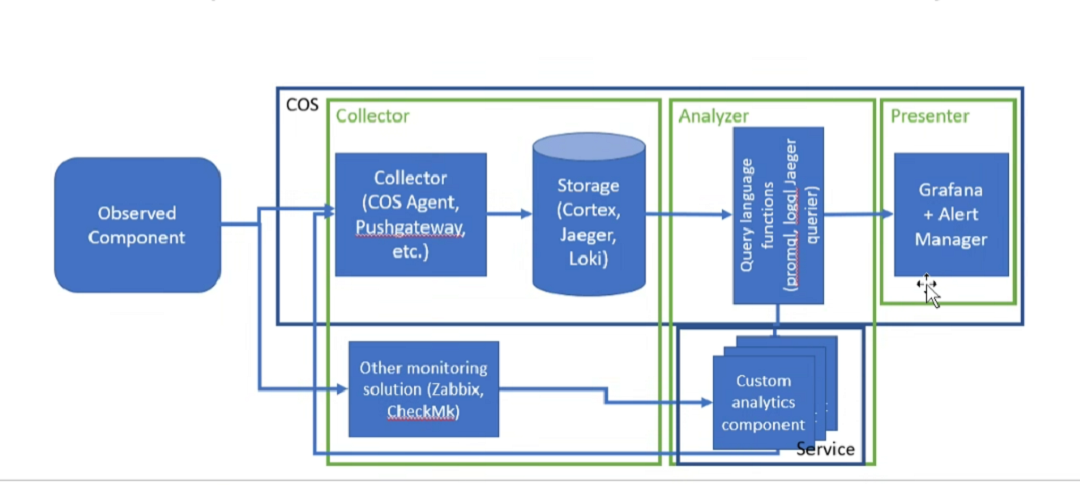
\includegraphics[width=1\linewidth]{img/rajz.png}
	\caption{Cos felépítése}
	\label{fig:cos_fel}
\end{figure}

